%&pdflatex
\documentclass[conference]{IEEEtran}
\usepackage{graphicx}
\usepackage{algorithm2e}
\usepackage[tight]{subfigure}
%\usepackage[sort&compress,numbers,merge]{natbib}

\begin{document}
\title{Forage RRT - An Efficient Approach To Task-Space Goal Planning for 
  Redundant Manipulators}
\author{%
  Leo Keselman\\ School of ECE\\ Georgia Institute of Technology\\
    L.D.Keselman@gmail.com \and
  Erik Verriest \\ School of ECE\\ Georgia Institute of Technology\\
    erik.verriest@ece.gatech.edu \and
  Patricio A. Vela\\ School of ECE\\ Georgia Institute of Technology\\
    pvela@ece.gatech.edu 
}
\maketitle

\newcommand{\CITE}{{\bf [CITE]}}

\begin{abstract}
Achieving efficient end-effector planning for manipulators in real world
workspaces is challenging due to the fact that planning is performed in
manipulator joint space, while the planning goal is given in end-effector or
tool space.  
For manipulator planning, the problem becomes a joint path
planning and inverse kinematics problem to be resolved efficiently, in spite
of the potentially infinite number of inverse solutions to the end-effector
goal state and the nonlinear relationship between joint configurations and
world obstacles.  The Forage-RRT algorithm described in this paper attempts
to efficiently and quickly resolve the end-effector or tool planning
problem.  Using ideas from foraging theory, Forage-RRT implements a
diffusion-based search strategy with two rates of diffusion, one high and
one low, which simulate both long jumps (coarse search) and focused small
area exploration (fine search) in the joint space, respectively.  During
coarse search, it is important to keep track of past fine searches,
therefore the traditional RRT algorithm is augmented with a goal heap that
keeps track of potential focused search regions and discards them when
they result in failure.  By mixing between two search distributions with
different spreads, the search space is rapidly covered and potentially
fruitful avenues are finely explored.  The search coverage advantages of
foraging identified in the biological research literature are demonstrated
here for end-effector based, manipulator path planning.  
\end{abstract}

%Modern planners can efficiently and rapidly identify paths when
%the initial state, the final state, and the planning states are all in
%the same space.  

\section{Introduction}
Task-based, manipulator motion planning algorithms seek to automatically and
quickly find a collision-free path in a general environment between any
given initial joint configuration (usually modeled by $R^m$ where $m$ is the
degrees of freedom of all the joints) and a goal point specified in 
end-effector or task space (a subspace of $SE(3)$).  Here, the goal is
specified in end-effector space because it is almost always the end-effector
(or tool) which interacts with the object to be manipulated. The specific
configuration of the final joint configuration is usually not important so
long as it is not in collision with workspace obstacles.  Examples of end
effector tools which interact with objects include hands, magnets, suction
cups, paint sprayers, and welders. Any practical manipulator planner has to
convert the given initial information into a trajectory fully residing in
joint space and meeting existing collision constraints.

The literature consists of two main approaches to solving the task-space
planning problem: either first solve end-effector goal directly using
inverse kinematics, or incorporate the search for the end-effector 
goal into planning.   Solving for a feasible inverse kinematics is difficult
due to the need to identify a goal joint configuration with collision-free
connectivity to the initial joint configuration.  To date, we are not
aware of an inverse kinematics algorithm for general n-link manipulators
which is complete, fast, and returns a configuration guaranteed to be
reachable from the start configuration.  Were it to exist, then the
task-space planning problem would be converted into a joint-space planning
problem with task-space obstacle constraints.  An efficient solution would
then be the bidirectional RRT \cite{lavalle00}, which is in the class of
Rapidly-Exploring Random Tree (RRT) algorithms, or any other solution
known to be fast (see \S \ref{sec:related}).

\paragraph{Problem Statement}
This paper tackles the second approach to task-space planning.  The initial
state is given in joint space.  The goal of the plan is expected to be 
specified as an end-effector configuration, either position only or position 
and orientation. The only assumptions are that the model of the manipulator
is known (at least enough to calculate a Jacobian) and that the world can be
queried to see if a given manipulator configuration would produce a
collision or not.  The task-space motion planner for (redundant) manipulators 
should be complete, single-query, and reliably fast for all reasonable
problems posed. 

\paragraph{Contribution}
The proposed solution, Forage-RRT, is an RRT algorithm with multiple 
diffusion rates and a greedy, goal-directed phase as part of planning.  
The main idea behind Forage-RRT is to initially explore the
manipulator space quickly with a large step-size RRT (high
diffusion rate) and then attempt to connect to the goal using a small
step-size RRT (low diffusion rate) from promising nodes in the large
step-size RRT. The algorithm alternates between the high and low diffusion
rate modes.  
To enable sensible greedy, goal-directed searches, the RRT is
augmented with a task-space goal heap (RRT+GH), which orders the RRT
joint space configurations via a heuristic score.  The ordering determines
which node will be used to initiate the greedy search.
Promising coarse step-size tree nodes are selected and removed from the goal 
heap, then used to initialize a small step-size RRT search.  
Forage RRT lends itself to parallel (or multi-core) implementation by
running several low-diffusion rate searches simultaneously.  We show that
Forage-RRT provides competitive average planning times that are further
improved through parallelization.  The result is a reliable planner which is
fast and consistent at solving a potentially wide range of manipulation
problems in environments with obstacles. 
%We believe the ease of implementing this approach along with its excellent
%performance on all problems will allow it to be used as a general
%manipulation planner both in industry and academia.

\paragraph{Organization}
The paper presents previous work we build upon as well as other
approaches to the same problem (\S \ref{sec:related}), 
an analysis of the shortcomings of the RRT in bug-trap problems 
(\S \ref{sec:bugtraprrt}), 
the implementation of the Forage-RRT algorithm (\S \ref{sec:implementation}), 
experiments and results compared to other planners having the same problem 
statement (\S \ref{sec:evaluation}), and 
finally a discussion of possible improvements to Forage-RRT (\S \ref{sec:disc}).  
\section{Related Work}
\label{sec:related}

Achieving tractable, complete motion planning for high dimensional 
systems such as (redundant) manipulators in general work environments
present several challenges. Algorithms to resolve the high-dimensional aspect 
have been the first to arise.  One of the most famous and most cited
approaches is the Artificial Potential Field Method originally presented in
\cite{khatib86}. Although this method is fast enough to be used in a single
query planner, it depends on obstacles being of a simple geometry and
suffers from several fundamental issues such as getting stuck in local
minima, no passage between closely spaced obstacles, and oscillations in
certain conditions \cite{koren91}.  Attempts have been made to solve these
issues by the formulation of new potential functions \cite{connolly90,ge00},
however, these functions either take prohibitively long to compute or do not
resolve all of the aforementioned pitfalls. 

Ariadne's Clew Algorithm \cite{bessiere93} approximates the feasible 
joint space via sampling. It uses an explore-search approach to achieve
resolution completeness and was shown to be respectably fast for most problems.
Algorithms based on probabilistic roadmaps \cite{amato96} use sampling 
to generate a roadmap for multi-query problems which allows subsequent
path planning problems to be solved efficiently.  Because the roadmap 
pre-processing step has a baseline overhead, it is not optimal for our stated 
goal of a single query planner for general environments.  Within the
category of efficient resolution-complete sampling based algorithms, the
Rapidly-Exploring Random Tree (RRT) family is popular and effective at solving 
many high dimensional planning problems \cite{lavalle98,lavalle00} 
For manipulation, standard RRTs depend on start and goal states given in joint 
space.  This bidirectional version \cite{lavalle00}, which grows two trees 
(sometimes randomly, sometimes toward each other), is effective in solving 
bug-trap problems. 
Since goals are most often not specified in joint space for manipulation
problems, a method for finding inverse kinematics algorithms to transform
the goal state into joint space is first needed
\cite{chang87,goldenberg85,guez88,parker89}. 
None of these inversion algorithms are complete and guaranteed to be
reachable from the start configuration. An inverse kinematics approach that
was guaranteed to return a configuration reachable from start was presented
in \cite{ahuactzin99}. 

When the planning problem also incorporates the inverse kinematics problem
as part of it, then the inverse kinematics solution will be resolution
complete and guaranteed reachable from the start. In \cite{bertram06}, the
RRT search is biased to be around the existing nodes which were closest in 
end-effector space to goal.  Significant speed improvements to the biased
search were achieved by using the Jacobian transpose or Jacobian 
pseudo-inverse to take steps in the direction of the goal from existing
nodes \cite{vahrenkamp09,vande07}.  Including such a bias is susceptible to 
getting stuck when the goal is occluded by an obstacle (similar to a
bug-trap).  Other RRT modifications include growing an additional
end-effector space tree which is then used to guide the growth of the
joint space tree \cite{diankov08,yao05}.  The former, \cite{diankov08},
grows the end-effector space tree from the goal in a bidirectional-type 
approach whereas the latter, \cite{yao05}, creates end-effector paths from 
start to goal. Both approaches struggle to find solutions quickly in 
bug-trap problems.
 
\section{RRT and the Bug-Trap Problem}
\label{sec:bugtraprrt}

\begin{figure}[h!]
  \centering
    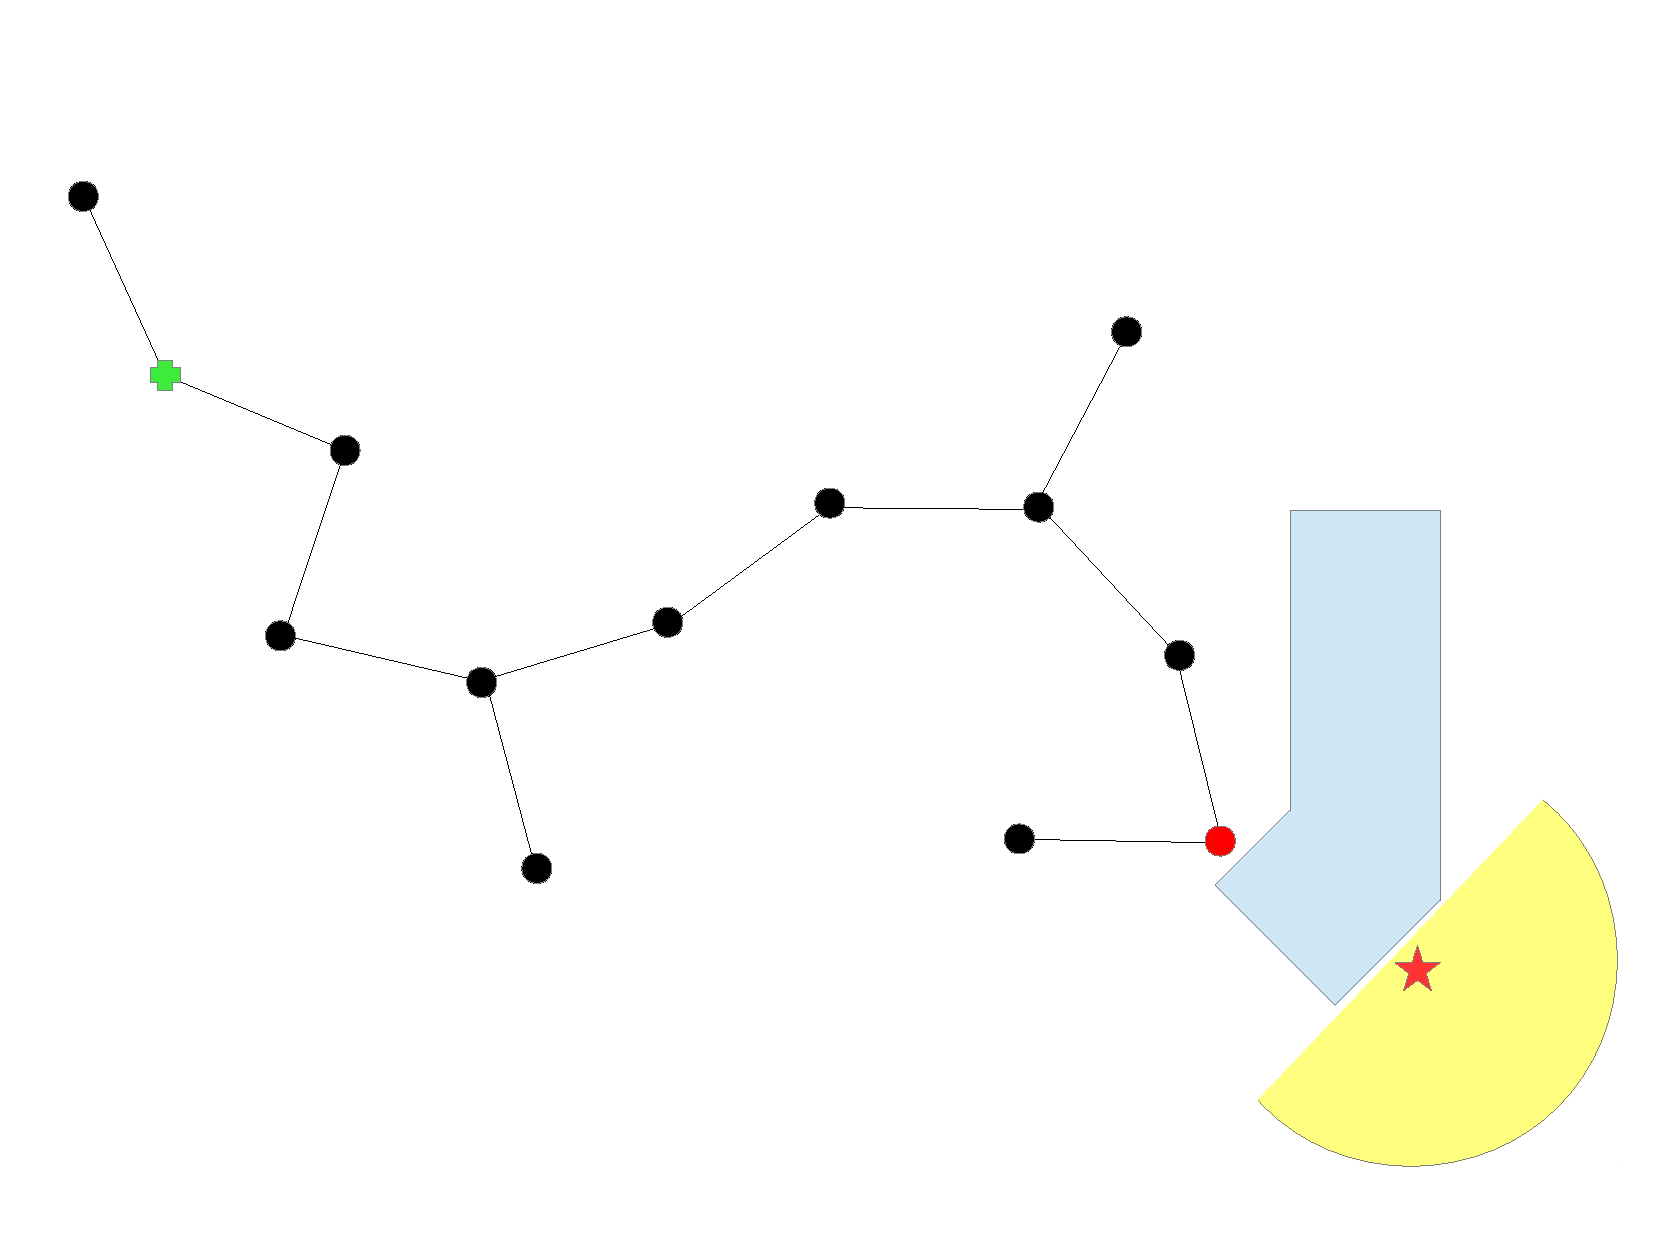
\includegraphics[width=0.4\textwidth]{figures/BugTrapRRT.pdf}
  \caption{An RRT attempting a bug-trap problem. \label{fig:BugTrapRRT} }
\end{figure}

Figure~\ref{fig:BugTrapRRT} shows an example of a uni-directional RRT 
attempting to solve a problem where the goal is occluded by an object.  The
state of the RRT is shown after 12 iterations of the extend operation (with
the probability of taking a step to goal being 35\%). At this state of the
tree, we can see that two problems emerge in our quest to connect the tree 
to the goal node:
\begin{enumerate}
\item Future attempts to step to goal will be taken from the red node since it is closest. All these attempts will fail because there is an
obstacle in the way, and are a waste of time.
\item To get to the goal, the RRT will have to find its way into the yellow
semicircle around the goal by virtue of only random steps. Any nodes outside
of this area will be either further than the red node or obstructed by the
obstacle. The probability of this happening quickly is very low.
Essentially, it would require that random configurations to extend toward
constantly be in the bottom right
corner of the workspace. For this simple example, the probability of getting
such random configurations looks to be around 1/15. In a different scenario
with a larger workspace and smaller step size, the probability would be
much smaller. 
\end{enumerate}

The important takeaway is that fast RRTs tend to approach the goal in a very 
directed fashion, but will be blocked by bug-trap type situations.  
Traditional RRTs rely on diffusion through random walks to go around
obstacles, but this process is slow for low probability situations.

\section{Forage RRT Implementation}
\label{sec:implementation}

The Forage-RRT algorithm, described in this section, utilizes ideas
from the biological foraging literature where it is shown that a
multi-diffusion rate process lowers the mean time to passage for foraging
problems \cite{Passino[2005],MoEtAl_JSM[2009]}.  The foraging problem is the
problem of finding a reward that has low probability of occurence in a large
space (with a penalty imposed on movement and searching).  The foraging
process model is a search process that has two diffusion rates (high and
low), that result in two modes of search, or at least two distinct movement
types\footnote{Some researchers prefer to use a single, heavy-tailed
distribution to generate the two movement types \cite{PlJa_JRSI[2008]}} 
(far and near, respectively).  By alternating between the two, search for an
unknown goal state in a large search space is faster than traditional
diffusion-based search, and covers a larger region versus greedy searches.
Each movement mode is also characterized as having a specific cost: low for
the high diffusion rate (far mode) and high for low diffusion rate (near
mode).  These costs are typically associated to the attention or energy
given to search versus movement. 

Forage-RRT replicates this idea within the context of our problem
statement.  The high diffusion rate mode utilizes a coarse step-size RRT
algorithm, with low probability of seeking the goal, and is akin to 
an exploration phase.  The low diffusion rate mode attempts to connect a node 
from the coarse tree to the goal via a fine step-size RRT algorithm with a
high probability of greedily seeking the goal.  The two RRTs have parameters
chosen to replicate the low/high attention characteristics found in
foraging.  The RRT in the fine-step/high-attention is more guided to the 
goal and will also more often use the manipulator Jacobian to move.  The
effect of this approach for bug-trap type problems is to solve the problem
presented in Section~\ref{sec:bugtraprrt} by using the coarse step-size tree
to cover joint space in search of promising approach directions to the goal,
then using the fine step-size tree to avoid any small occlusions that remain
on the path to the goal.

\subsection{Goal Heap}
An inefficiency in the basic RRT algorithm is that unsuccessful steps to
goal may continuously be taken from the same node because that node is the
closest to goal, as illustrated in \S\ref{sec:bugtraprrt}.
%In RRT implementations for static environments, it is unnecessary and
%inefficient to continue to attempt steps to goal from nodes from which such
%a step has already been attempted - if it did not reach goal before, it will
%not again.  
Our solution to the problem is to implement a goal heap. 
When new nodes are added to the RRT, they are also added to the goal heap
along with their value (some heuristic that evaluates the fitness of the
joint state with regards to proximity to goal). In our case, the value of a
node was simply the inverse of its Euclidean distance to goal position. The
heap data structure automatically orders the nodes by value so that the top
of the heap is the highest value node. Once a step to goal is attempted from
a node, that node is removed from the goal heap because using it again for a
step to goal would be a fruitless endeavor.  While the goal heap can apply
to any RRT implementation, it is essential for the Forage RRT because the
heap provides a node in the coarse tree for use when attempting a fine 
step-size J+RRT to connect to goal.

\subsection{RRT Extend Implementations}
Both coarse and fine RRT implementations use the J+RRT algorithm 
\cite{vahrenkamp09} with the proposed goal heap augmentation (J+RRT+GH).  
Random extensions of the search tree use the
standard extension procedure of picking a random point in joint space and
taking a step towards it from the nearest neighbor already in the tree. 
Goal-directed extensions use the Moore-Penrose pseudo-inverse Jacobian to 
take a step in the proper direction.  The overall extend implementation is 
shown in Algorithm~\ref{alg:extend}. 

\paragraph{Coarse versus fine search.}
The coarse search should focus more on rapidly exploring the space rather
than seeking the goal.  This is done by lowering the probability of stepping
to goal in the coarse J+RRT+GH implementation, which also lowers the
exploration cost.  Since the coarse J+RRT+GH takes large step sizes, for each
node extension, the link between the new node and its parent must be checked 
for validity by iterating through its length at an acceptable resolution and 
making sure each smaller step is valid.  In contrst, the fine search should 
focus on exploring a small region with a greater intent to find the final
goal state.  The fine J+RRT implementation has a higher probability of
stepping to goal.  For the fine step-size J+RRT+GH, we assume that if the new
node is valid, then the path connecting the parent node to the new node is
also valid. 

\begin{algorithm}
  \label{alg:extend}
  \SetAlgoLined
  \KwData{$RRT, goal, StepSize$}
  \KwResult{$Updated RRT, StepResult$} 

  $\rho \leftarrow random([0,100])$\;
  \eIf{$\rho < randomExtendProbability$}
   {
    $x_{rand} \leftarrow RANDOM\_STATE()$\;
    $x_{near} \leftarrow NEAREST\_NODE(x_{rand}, RRT)$\;
    $x_{new} \leftarrow TAKE\_STEP(x_{rand}, x_{near}, StepSize)$\;
    \eIf{$isLegalPath(x_{near},x_{new})$}
	 {
      $RRT \leftarrow addVertex(x_{new})$\;
      $RRT \leftarrow addEdge(x_{near}, x_{new}, StepSize)$\;
      $NodeValue \leftarrow value(x_{new})$\;
      $GoalHeap \leftarrow insert(x_{new}, NodeValue)$\;
      \eIf{$x_{new} = x_{randomConfig}$}
	   {
        $return \; STEP\_REACHED$\;
       }{
        $return \; STEP\_PROGRESS$\;
       }
     }{
       $return \; STEP\_COLLISION$\;
     }	
   }{	
    $x_{near} \leftarrow GoalHeap \rightarrow top$\;
    $x_{new} \leftarrow JAC\_STEP(x_{near}, goal, StepSize)$\;
    \eIf{$isLegalPath(x_{near},x_{new})$}
	 {
      $RRT \leftarrow addVertex(x_{new})$\;
      $RRT \leftarrow addEdge(x_{near}, x_{new}, StepSize)$\;
      \eIf{$x_{new} = goal$}
	   {
        $return \; GOAL\_REACHED$\;
       }{
        $NodeValue \leftarrow value(x_{new})$\;
        $GoalHeap \leftarrow insert(x_{new}, NodeValue)$\;
        $GoalHeap \leftarrow remove(x_{near})$\;
        $return \; STEP\_PROGRESS$\;
       }	
     }{
       $GoalHeap \leftarrow remove(x_{near})$\;
       $return \; STEP\_COLLISION$\;
     }
   }
  \caption{J+RRT+GH Extend Operation}
\end{algorithm}

\subsection{Foraging: Alternating Between Explore and Search}
The main Forage RRT algorithm is shown in Algorithm~\ref{alg:ForageRRT}. The
first while loop initially explores the space and builds up several promising 
nodes to initialize the fine searches with. The second while loop searches
by attempting to connect the promising nodes from the coarse step-size tree
to the goal with a fine step-size tree. Once a fine step-size RRT
experiences a certain number of collisions, we give up on it and try to
start another one from the next most promising node. After a given number of
fine step-size searches fail, grow the coarse step-size tree (e.g.,
return to explore mode) to replenish the heap with promising start nodes.
The finite search cost and restarts from alternative promising nodes allows
us to make the fine step-size RRT greedy, making it fast in easy situations
but also robust to more challenging situations. A full list of parameters we
used is given in Section~\ref{sec:evaluation}.

Once the fine step-size RRT has reached the goal, the found path is obtained
by tracing to the root of the fine step-size tree, which is a node in the
coarse step-size tree, then tracing to the root of the coarse step-size tree.
Due to the mixed step-size RRTs, the raw final plan will not be attractive, 
especially near the start. For this purpose, path smoothing is required to 
make the path acceptable. This is done in a quick manner by taking pairs of
nodes, attempting to connect them with a straight line, and deleting all
nodes in between if successful. Empirically, we have found that
picking a node from the coarse step-size plan and trying to connect it to 
the fine step-size plan works well.  The second step is to go through
remaining coarse steps and subdivide them into the desired step size to
match the rest of the path.  We have found that 15-20 successful smoothing 
steps result in a smooth path.  The computational cost for path smoothing is
low compared to the path planning procedure.

\begin{algorithm}
  \label{alg:ForageRRT}
  \SetAlgoLined
  \KwData{start, goal}
  \KwResult{path from start to goal}
  $CoarseRRT \leftarrow INIT(largeStepSize, start, goal)$\;
  \While{$CoarseRRT \rightarrow size < initialSize$}
   {
	$CoarseRRT \rightarrow EXTEND()$\;
   }
  \While{$result \neq GOAL\_REACHED$}
   {
    $numFailures \leftarrow 0$\;
	$FineRRT \leftarrow INIT(fineStepSize, 
	                         CoarseRRT \rightarrow GoalHeap \rightarrow top)$\;
	\While{$numCollisions < maxNumCollisions$}
	 {
	  $FineRRT \rightarrow EXTEND()$\;
	 }
	increment $numFailures$ \;
	\If{numFailures = maxNumFailures}
	 {
	  \For{1:percentIncrease*initialSize}
	   {
		$CoarseRRT \rightarrow EXTEND()$\;
	   }
	 }
   }
  \caption{Forage-RRT}
\end{algorithm}

\subsection{Parallel Implementation}
The two search strategies in Forage-RRT are parellelizable.
Using a Master-Worker parallel implementation, the main steps are:
\begin{itemize}
  \item \textbf{Initial Step: } 
	Grow coarse step-size tree to an initial size greater than the number of
	threads to be used.
  \item \textbf{Worker Threads: } 
	Grow a fine step-size tree to goal with a seeded start configuration from 
	the coarse step-size tree. Terminate upon success or when a certain 
	number of collisions occur.
  \item \textbf{Master Thread: } 
    1) Grow coarse step-size RRT; 
	2) Maintain worker threads by seeding them with the best available node 
	  from coarse step-size RRT when they terminate without success.
\end{itemize}

\section{Experiments and Evaluation}
\label{sec:evaluation}
\subsection{Experiments}
\subsubsection{Sequential Implementation}
Experiments were conducted on a Schunk 7 DOF arm with the DART/GRIP
simulator (developed by the GOLEMS lab at Georgia Tech) on a 2.27GHz, 8 core
machine. We compared the following algorithms to the path-smoothed Forage-RRT:
\begin{enumerate}
  \item RRT-JT \cite{vande07}
  \item J+RRT with goal directed steps \cite{vahrenkamp09} 
  \item BiSpace RRT \cite{diankov08}
  \item Kinematic Roadmap \cite{ahuactzin99}. The paths produced 
    from this algorithm would be too long to be used for most applications. 
	Rather only the inverse kinematics solution, which is guaranteed to be 
	reachable from start, would be used.
\end{enumerate}

\begin{figure*}[t]
  \centering
  \subfigure[Easy case for testing: no obstacles.]
   	{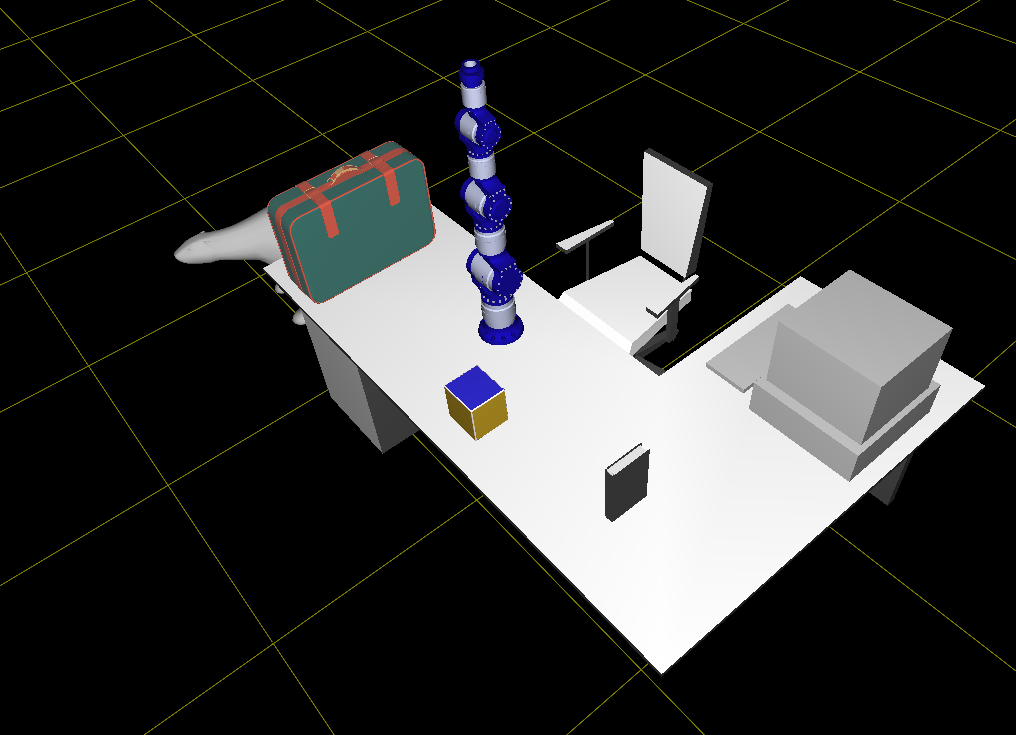
\includegraphics[width=0.29\textwidth]{figures/EasyCase.png}}
  \subfigure[Medium case for testing: obstacles throughout space.]
    {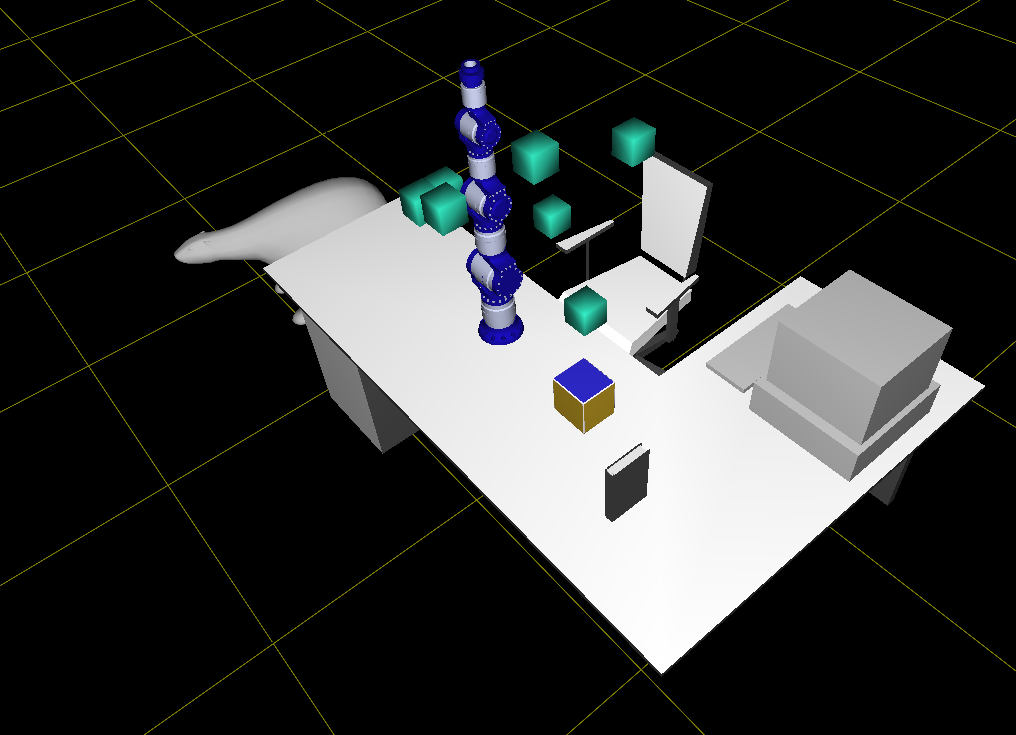
\includegraphics[width=0.29\textwidth]{figures/MediumCase.png}}
  \subfigure[Hard case for testing: goal directly under obstacle, near edge of workspace ]
   	{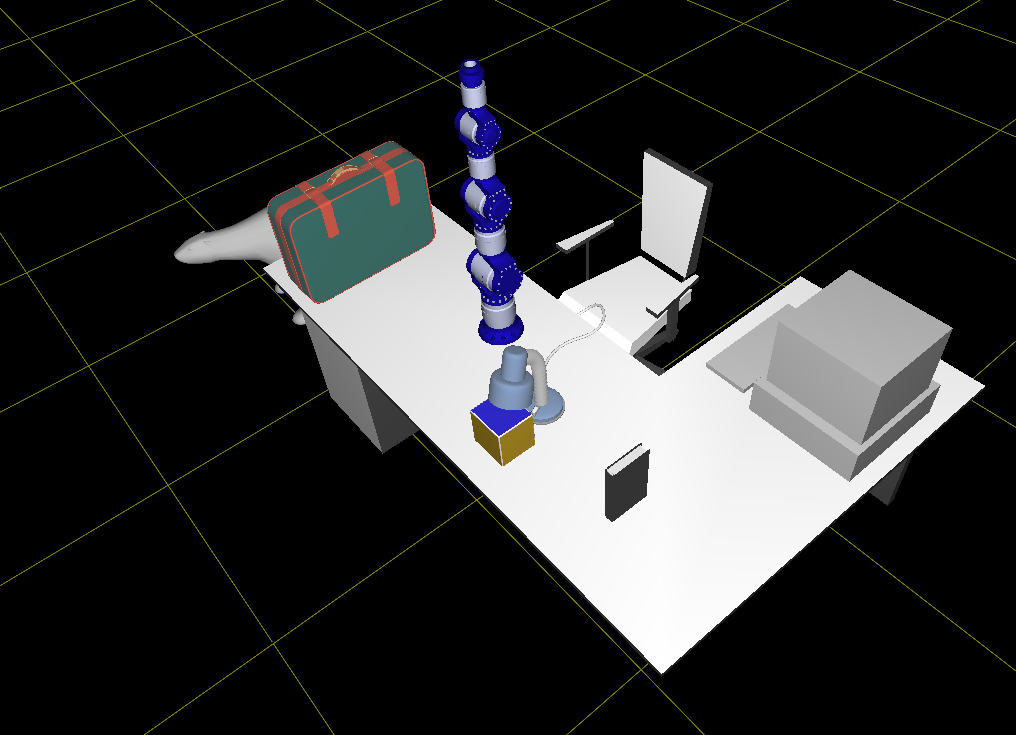
\includegraphics[width=0.29\textwidth]{figures/HardCase.png}}
  \caption{Depiction of different test cases.}
  \label{fig:cases}
\end{figure*}

The smoothing time was included in Forage RRT results but not for the other 
results because the paths produced did not strictly require it. Moreover,
any RRT reaching 10,000 nodes was restarted to improve the average planning
time of all planners (empirically it seems that an RRT that grows too large
will have trouble connecting to the goal, so it is better to restart).
The Forage-RRT parameters used for testing are given in
Table~\ref{tab:ForageParams} (with common parameters for the other
algorithms equaling those from the table).

Each algorithm was tested on an easy, medium, and hard case. Figure 
(\ref{fig:cases}) depicts the cases.  The goal is the point where the three 
shown faces of the gold and blue cube meet. 50 random collision-free start 
configurations were computed for each case (easy, medium, and hard) and the 
same 50 start configurations were used for each algorithm. Each start 
configuration was the seed for 40 runs, thus totaling 2000 runs per
algorithm per case. In the interest of time, a run was considered a failure
if the RRT had to be restarted 25 times and no solution was found (such
a run would have taken 400-600 seconds so it should be penalized). 

\begin{table}
  \centering
  \caption{Forage RRT parameters. \label{tab:ForageParams}}
  \begin{tabular}{| c | c | }
    \hline
	initialSize & 50 \\ \hline
  	randomExtendProbability - coarse & 90 \\ \hline
  	randomExtendProbability - fine & 65 \\ \hline
  	largeStepSize & 1.3\\ \hline
  	fineStepSize & .02\\ \hline
  	maxNumCollisions & 5\\ \hline
  	maxNumFailures & 10\\ \hline
	percentIncrease & .25\\ \hline 
  \end{tabular}
\end{table}

\subsubsection{Parallel Implementation}
To test the parallel algorithm, experiments were conducted on the same cases
as the sequential Forage-RRT. The parallel implementations were tested for
10 precomputed start configurations per case, at 40 runs per start
configuration. Thus, each version was tested 400 times. The implementation
was tested with one to six worker threads. 

\subsection{Evaluation}

\subsubsection{Sequential Implementation}
The results of the sequential implementation simulation are shown in 
Table~\ref{tab:Results}. The reported times are averaged over completed
cases only.  For all cases, the Forage-RRT provided the lowest average
completion time and also maintained a 100\% completion rate for the tasks.

\begin{table*}
  \caption{Sequential experiment results. All times in seconds. 
    \label{tab:Results}}
  \centering
  \begin{tabular}{| c | c | c | c | c | c | c | }
  \hline
  Algorithm & \textbf{Easy Avg} & \textbf{\% Comp} &\textbf{Med Avg} & 
             \textbf{\% Comp} & \textbf{Hard Avg} & \textbf{\% Comp} \\ \hline
  \textbf{Forage RRT}&
  \textbf{2.92}&\textbf{100}&\textbf{3.01}&\textbf{100}&\textbf{7.52}&
  \textbf{100}\\ \hline
  \textbf{RRT-JT}& 12.12&93.7&30.51&82.7&62.62&29.0\\ \hline
  \textbf{Jinv-RRT}&4.45&96.9&21.42&92.0&65.92&53.6\\ \hline
  \textbf{BiSpace RRT}&4.57&100&21.94&99.96&36.87&80.6\\ \hline
  \textbf{Kin. Roadmap}&5.22&100&4.72&100&22.21&100\\ \hline
\end{tabular}
\end{table*}

\subsubsection{Parallel Implementation}
The results of the parallel implementation for the tested number
worker threads are shown in Figure~\ref{fig:ParallelResults}. 
The decline in search time is sub-linear.  Because the solution is often 
found in the first few attempts to connect to goal from the coarse RRT, we
hypothesize that additional threads beyond a certain amount will initiate a 
fine search that will not be needed.
For our experiments, the results imply that improvements after four working 
threads would be minimal. The best average planning times achieved with the 
parallel implementation are summarized in Table~\ref{tab:BestParallel} and 
apply to the case when four worker threads were implemented.

\begin{figure}[h!]
  \centering
    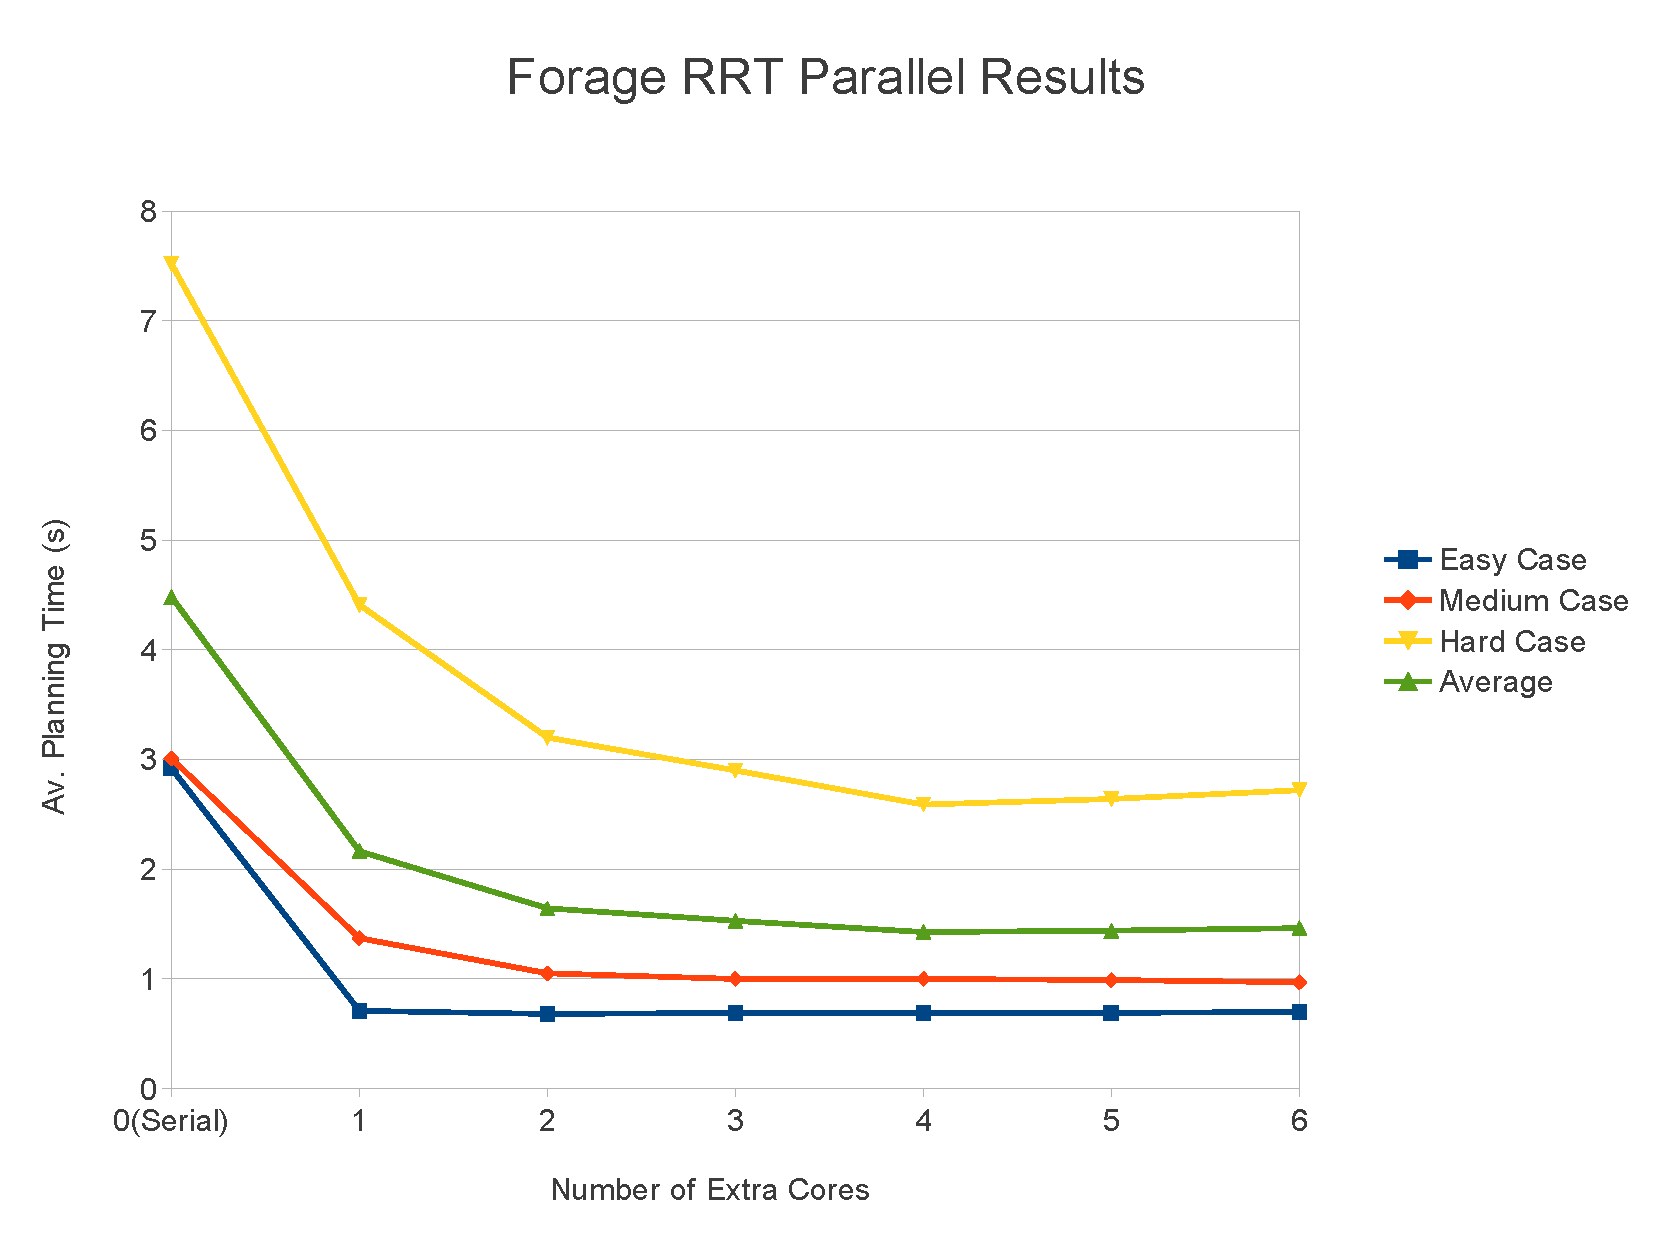
\includegraphics[width=0.45\textwidth]{figures/ParallelGraph.pdf}
  \caption{Average planning times per number of extra cores used. 
    \label{fig:ParallelResults} }
\end{figure}

\begin{table}
  \centering
  \caption{Parallel (4 core) planning results. All times in seconds.
    \label{tab:BestParallel}}
  \begin{tabular}{|c|c|c|c|c|}
    \hline
    Case: & easy & Medium & Hard & Average \\
	\hline
	Avg. Time: & .69 & 1.00 & 2.59 & \textbf{1.43} \\  \hline
  \end{tabular}
\end{table}

\section{Discussion}
The benefits of the Forage-RRT arise from the two different diffusion rates
associated to the two RRT implementations.  For the purpose of visualization, 
the end-effector positions of a sample, initial coarse RRT are shown in 
Figure~\ref{fig:CoarseRRT}.  
The green node is the start and the red node is the goal.
The closest nodes to the goal come from many different directions, making
the fine RRTs more likely to be effective.

\begin{figure}[h!]
  \centering
  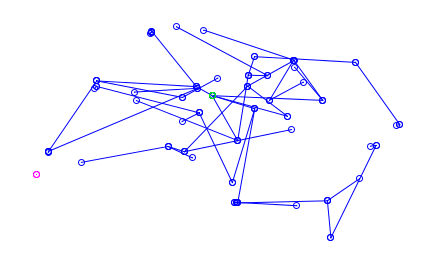
\includegraphics[width=0.35\textwidth]{figures/coarseRRTExample.png}
  \caption{End-effector positions for an initial coarse RRT. 
    \label{fig:CoarseRRT} }
\end{figure}

\label{sec:disc}
\subsection{Completeness}
From \cite{lavalle98}, any RRT is resolution complete because its
coverage of the workspace converges to the sampling distribution.  Because
the coarse RRT in the Forage-RRT algorithm searches indefinitely, the 
Forage-RRT is also resolution complete. Needless to say, it is highly
unlikely in practice that the coarse step-size tree will be the one to come
upon the goal.

\subsection{Parameters}
The Forage RRT parameters used to achieve the results in
Table~\ref{tab:Results} are given in Table~\ref{tab:ForageParams}. These
parameters were arrived at empirically by running a few test cases, 
and are not guaranteed to be ideal ones. It may be of interest to
investigate ideal values for these parameters, for instance when to switch
from fine searching to coarse searching. Perhaps there should be a
heuristic function rather than a hard constraint on failures. Moreover, 
parameters such as initial coarse tree size and the coarse step-size may be 
good candidates for learning over time. We conjecture that the ideal
values for these parameters depend on specific environment factors such as
the obstacle density and obstacle geometry. 
%The Forage-RRT algorithm
%presented in Section~\ref{sec:implementation} should be a very strong base
%line for any motion planning environment, especially one for a manipulator,
%but improvements could foreseeably be made to make it more adaptible to any
%environment.

%\subsection{Replanning}
%In situations where the environment has changed but the start and goal have
%not, the Forage RRT lends itself to possible future work in replanning
%strategies. For instance, it may be faster to modify the parts of the coarse
%tree affected by the environment changes than to rebuild the whole tree from
%scratch.  Another idea may be to reuse the coarse node which was a
%successful start for the fine RRT in the previous run as a waypoint in the
%search to bias the tree toward an area which is likely to be successful
%again.  

\section{Conclusion}
We have presented the Forage-RRT algorithm for motion planning. The premise
behind the algorithm is that a foraging-based search algorithm provides an 
excellent compromise between diffusion-based searching (via random samples) 
and greedy search (goal-directed movements) in single-query, task-based, 
manipulator planning algorithms.  The effectiveness of the method has been
shown through randomized trials on scenarios with variable difficulty.

%We believe the algorithm's efficieny on tough problems, consistency,
%completeness, ease of implementation, and parallel potetial make it the best
%available motion planning algorithm for general problems where the goal is
%specified in task space. We have shown its effectiveness specifically for
%redundant manipulators.

\paragraph{Acknowledgments} This work was supported in part by the National
Science Foundation (ECS-0238993).

\bibliographystyle{IEEEtran}
\bibliography{RRT,MotionPlanning,IK}

\end{document}

